% Appendix A

\chapter{Modelo de datos del warehouse} % Main appendix title

\label{AppendixA}

En este apéndice se describen las tablas y vistas del warehouse \code{WH\_PSYD} que intervienen en el pipeline de datos presentado en la sección~\ref{sec:pipeline_datos}. Se detallan los esquemas DEMANDA, METEO y PRONOS, junto con las dimensiones que los vinculan. Para cada objeto se indican la capa a la que pertenece, su clave y su contenido. Las variables comunes a varias tablas se describen una única vez.

%----------------------------------------------------------------------------------------
\section{Relaciones entre esquemas}
\label{sec:apendice_relaciones}
%----------------------------------------------------------------------------------------

Los esquemas se vinculan mediante tres identificadores. \code{RGE\_ID} identifica las regiones eléctricas, definidas en la tabla \code{REGIONES\_ELECTRICAS\_TOTALES} del esquema \code{GENERAL}. Luego, \code{EMET\_ID} identifica las estaciones meteorológicas, y \code{PRON\_ID} identifica los modelos y servicios de pronóstico. Las tablas de dimensiones incluyen períodos de vigencia (\code{FECHA\_DESDE} y \code{FECHA\_HASTA}), por lo que las vistas de capa~3 asocian cada estación con su región según la fecha del dato. La figura~\ref{fig:modelo_datos} resume estas relaciones.

\begin{figure}[H]
	\centering
	\resizebox{\textwidth}{!}{%
		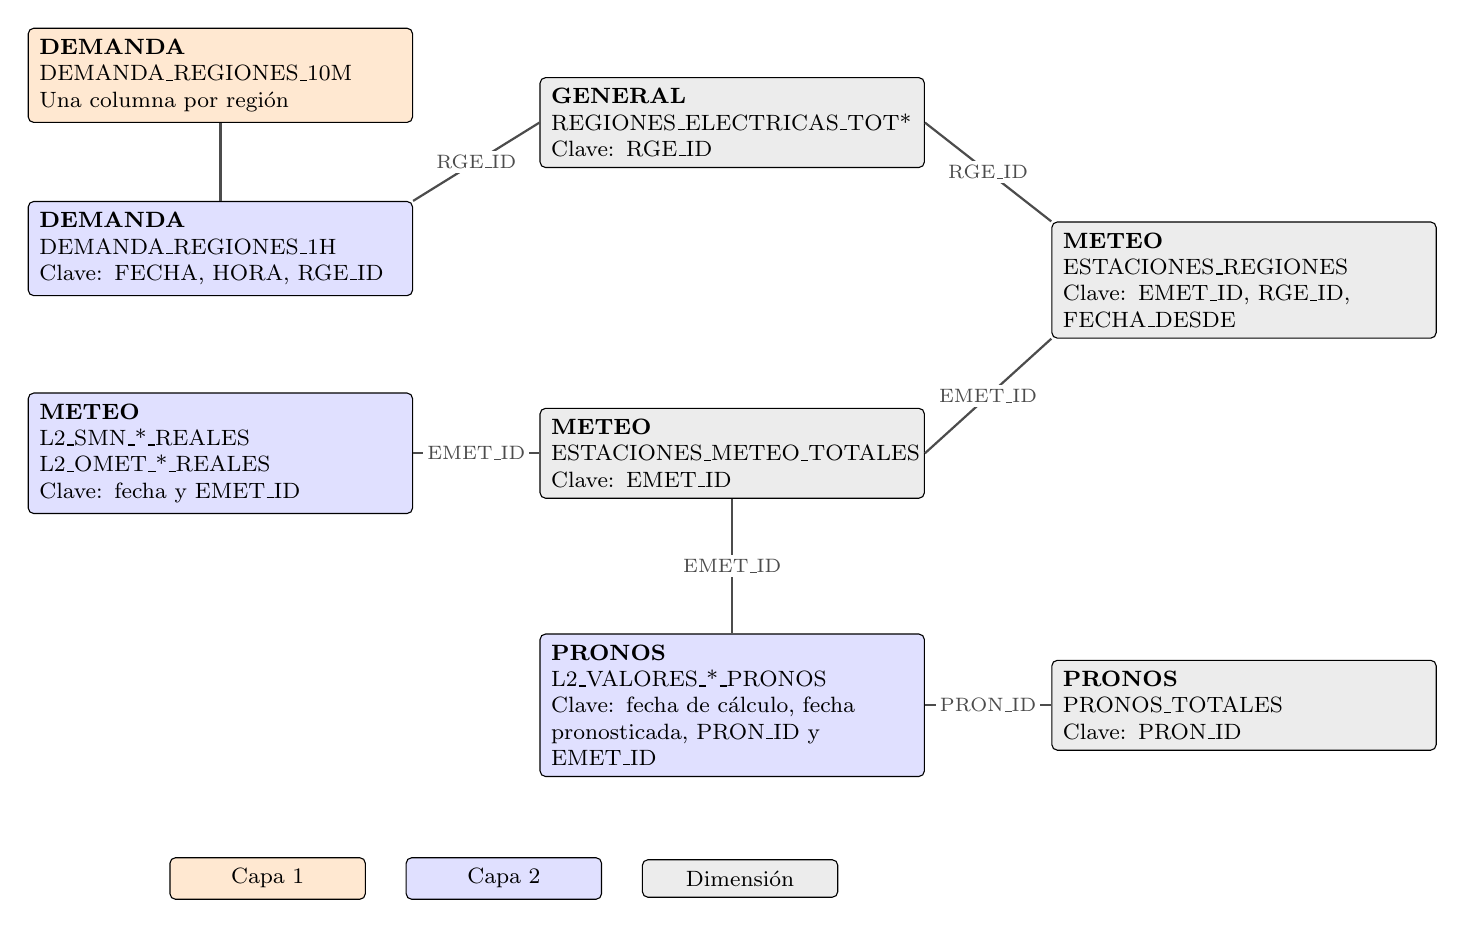
\begin{tikzpicture}[
			font=\footnotesize,
			tabla/.style={draw, rounded corners=2pt, align=left, text width=4.6cm, inner sep=4pt},
			dimension/.style={tabla, fill=gray!15},
			capados/.style={tabla, fill=blue!12},
			capauno/.style={tabla, fill=orange!18},
			vista/.style={tabla, fill=green!14},
			rel/.style={thick, gray!60!black},
			clave/.style={font=\scriptsize, fill=white, inner sep=1.5pt}
			]
			% Dimensiones
			\node[dimension] (reg) at (6.5,1) {\textbf{GENERAL}\\\code{REGIONES\_ELECTRICAS\_TOT*}\\Clave: \code{RGE\_ID}};
			\node[dimension] (est) at (6.5,-3.2) {\textbf{METEO}\\\code{ESTACIONES\_METEO\_TOTALES}\\Clave: \code{EMET\_ID}};
			\node[dimension] (er) at (13,-1.0) {\textbf{METEO}\\\code{ESTACIONES\_REGIONES}\\Clave: \code{EMET\_ID}, \code{RGE\_ID}, \code{FECHA\_DESDE}};
			\node[dimension] (pt) at (13,-6.4) {\textbf{PRONOS}\\\code{PRONOS\_TOTALES}\\Clave: \code{PRON\_ID}};
			% Hechos
			\node[capauno] (d10) at (0,1.6) {\textbf{DEMANDA}\\\code{DEMANDA\_REGIONES\_10M}\\Una columna por región};
			\node[capados] (d1h) at (0,-0.6) {\textbf{DEMANDA}\\\code{DEMANDA\_REGIONES\_1H}\\Clave: \code{FECHA}, \code{HORA}, \code{RGE\_ID}};
			\node[capados] (ml2) at (0,-3.2) {\textbf{METEO}\\\code{L2\_SMN\_*\_REALES}\\\code{L2\_OMET\_*\_REALES}\\Clave: fecha y \code{EMET\_ID}};
			\node[capados] (pl2) at (6.5,-6.4) {\textbf{PRONOS}\\\code{L2\_VALORES\_*\_PRONOS}\\Clave: fecha de cálculo, fecha pronosticada, \code{PRON\_ID} y \code{EMET\_ID}};
			% Relaciones
			\draw[rel] (d1h.north east) -- (reg.west) node[clave, midway] {\code{RGE\_ID}};
			\draw[rel] (d10.south) -- (d1h.north);
			\draw[rel] (ml2.east) -- (est.west) node[clave, midway] {\code{EMET\_ID}};
			\draw[rel] (est.east) -- (er.south west) node[clave, midway] {\code{EMET\_ID}};
			\draw[rel] (reg.east) -- (er.north west) node[clave, midway] {\code{RGE\_ID}};
			\draw[rel] (pl2.north) -- (est.south) node[clave, midway] {\code{EMET\_ID}};
			\draw[rel] (pl2.east) -- (pt.west) node[clave, midway] {\code{PRON\_ID}};
			% Leyenda
			\node[capauno, text width=2.2cm, align=center] at (0.6,-8.6) {Capa 1};
			\node[capados, text width=2.2cm, align=center] at (3.6,-8.6) {Capa 2};
			\node[dimension, text width=2.2cm, align=center] at (6.6,-8.6) {Dimensión};
		\end{tikzpicture}%
	}
	\caption{Relaciones entre las tablas principales de los esquemas DEMANDA, METEO y PRONOS.}
	\label{fig:modelo_datos}
\end{figure}

%----------------------------------------------------------------------------------------
\section{Esquema DEMANDA}
\label{sec:apendice_demanda}
%----------------------------------------------------------------------------------------

El esquema DEMANDA contiene la demanda eléctrica calculada a partir del SOTR y las variables objetivo de los modelos. La tabla~\ref{tab:esquema_demanda} describe sus objetos.

\begin{table}[H]
	\centering
	\caption{Tablas y vistas del esquema DEMANDA.}
	\label{tab:esquema_demanda}
	\footnotesize
	\setlength{\tabcolsep}{4pt}
	\renewcommand{\arraystretch}{1.15}
	\begin{tabularx}{\textwidth}{
			@{}
			>{\raggedright\arraybackslash\hsize=1.1\hsize}X
			>{\raggedright\arraybackslash\hsize=0.6\hsize}X
			>{\raggedright\arraybackslash\hsize=0.9\hsize}X
			>{\raggedright\arraybackslash\hsize=1.4\hsize}X
			@{}
		}
		\toprule
		\textbf{Objeto} & \textbf{Tipo y capa} & \textbf{Clave} & \textbf{Contenido} \\
		\midrule
		\code{DEMANDA\_} \code{REGIONES\_10M} & Tabla, capa~1 & \code{FECHA}, \code{HORA}, \code{INTERVALO} &
		Demanda en MW cada diez minutos, en formato ancho, con una columna por región y otra para el MEM, junto con las variables de control del cálculo. \\ \addlinespace
		\code{DEMANDA\_} \code{REGIONES\_1H} & Tabla, capa~2 & \code{FECHA}, \code{HORA}, \code{RGE\_ID} &
		Demanda horaria depurada por región, con el valor original anterior a la limpieza y la marca de corrección. \\ \addlinespace
		\code{DEMANDAS\_MEM} & Vista, capa~3 & \code{FECHA}, \code{TARGET\_} \code{ID\_ASOCIADO} &
		Variables objetivo diarias del MEM: energía (1), potencia máxima entre las 6 y las 24 horas (2) y potencia mínima entre las 0 y las 12 horas (3). \\
		\bottomrule
	\end{tabularx}
\end{table}

La tabla~\ref{tab:columnas_demanda} detalla las columnas de las dos tablas del esquema.

\begin{table}[H]
	\centering
	\caption{Columnas de las tablas del esquema DEMANDA.}
	\label{tab:columnas_demanda}
	\footnotesize
	\setlength{\tabcolsep}{4pt}
	\renewcommand{\arraystretch}{1.15}
	\begin{tabularx}{\textwidth}{
			@{}
			>{\raggedright\arraybackslash\hsize=0.8\hsize}X
			>{\raggedright\arraybackslash\hsize=1.2\hsize}X
			@{}
		}
		\toprule
		\textbf{Columna} & \textbf{Descripción} \\
		\midrule
		\multicolumn{2}{@{}l}{{\textbf{Tabla \code{DEMANDA\_} \code{REGIONES\_10M}}}} \\
		\code{FECHA}, \code{HORA}, \code{INTERVALO} & Fecha, hora e intervalo de diez minutos de la medición. \\
		\code{MEM} & Demanda del MEM, calculada como suma de las regiones, en MW. \\ \\
		\code{GBA}, \code{CEN}, \code{LIT}, \code{CUY}, \code{NEA}, \code{NOA}, \code{COM}, \code{PBN}, \code{PBS}, \code{PAT} & Demanda de cada región eléctrica corregida por pérdidas, en MW. \\ \\
		\code{CHK\_MEM\_TAG}, \code{CHK\_MEM\_DIF}, \code{CHK\_MEM\_DIF\_PORC} & Medidor nacional de referencia y diferencias absoluta y porcentual respecto del MEM calculado. \\ \\
		\code{CHK\_PBA}, \code{CHK\_PBN\_TAG}, \code{CHK\_PBS\_TAG}, \code{CHK\_PBA\_PARTICION}, \code{CHK\_DIF\_PBN}, \code{CHK\_DIF\_PBS}, \code{CHK\_DIF\_PBN\_PORC}, \code{CHK\_DIF\_PBS\_PORC} & Controles de la partición de PBA: demanda original de la región, mediciones directas de PBN y PBS y diferencias absolutas y porcentuales asociadas con la partición. \\ \\
		\code{CHK\_INTERCAMBIOS} & Suma de los intercambios entre regiones, que debe permanecer próxima a cero. \\ \addlinespace
		\multicolumn{2}{@{}l}{{\textbf{Tabla \code{DEMANDA\_REGIONES\_1H}}}} \\
		\code{FECHA}, \code{HORA} & Fecha y hora, con la convención horaria de CAMMESA (1 a 24). \\
		\code{RGE\_ID} & Identificador de la región eléctrica. \\
		\code{VALOR} & Demanda horaria depurada, en MW. \\
		\code{VALOR\_ORIGINAL} & Demanda horaria calculada con los datos anteriores a la limpieza, en MW. \\
		\code{FLAG\_CORREGIDO} & Indica si \code{VALOR} difiere de \code{VALOR\_ORIGINAL}. \\
		\bottomrule
	\end{tabularx}
\end{table}

%----------------------------------------------------------------------------------------
\section{Esquema METEO}
\label{sec:apendice_meteo}
%----------------------------------------------------------------------------------------

El esquema METEO contiene las estaciones meteorológicas, su asociación con las regiones eléctricas y los datos observados del SMN y de Open-Meteo. La tabla~\ref{tab:esquema_meteo} describe sus objetos. Las tablas de capa~2 se separan por fuente y por resolución, mientras que las vistas de capa~3 integran ambas fuentes: para cada variable toman el valor del SMN y, si no está disponible, el de Open-Meteo.

\begin{table}[H]
	\centering
	\caption{Tablas y vistas del esquema METEO.}
	\label{tab:esquema_meteo}
	\footnotesize
	\setlength{\tabcolsep}{4pt}
	\renewcommand{\arraystretch}{1.15}
	\begin{tabularx}{\textwidth}{
			@{}
			>{\raggedright\arraybackslash\hsize=1.3\hsize}X
			>{\raggedright\arraybackslash\hsize=0.55\hsize}X
			>{\raggedright\arraybackslash\hsize=0.75\hsize}X
			>{\raggedright\arraybackslash\hsize=1.4\hsize}X
			@{}
		}
		\toprule
		\textbf{Objeto} & \textbf{Tipo y capa} & \textbf{Clave} & \textbf{Contenido} \\
		\midrule
		\code{ESTACIONES\_METEO\_\allowbreak TOTALES} & Dimensión & \code{EMET\_ID} &
		Estaciones meteorológicas: nombre, código OACI, provincia, región y prioridad dentro de ella, coordenadas, altura, localidad del SMN y vigencia. \\ \addlinespace
		\code{ESTACIONES\_REGIONES} & Dimensión & \code{EMET\_ID}, \code{RGE\_ID} &
		Estación representativa de cada región eléctrica y su período de vigencia. \\ \addlinespace
		\code{L2\_SMN\_\allowbreak VALORES\_HORARIOS\_\allowbreak REALES} & Tabla, capa~2 & \code{FECHA\_HORA}, \code{EMET\_ID} &
		Observaciones horarias del SMN y temperatura aparente calculada. \\ \addlinespace
		\code{L2\_SMN\_\allowbreak VALORES\_DIARIOS\_\allowbreak REALES} & Tabla, capa~2 & \code{FECHA}, \code{EMET\_ID} &
		Valores diarios del SMN, sin nubosidad, precipitación ni radiación. \\ \addlinespace
		\code{L2\_OMET\_\allowbreak VALORES\_HORARIOS\_\allowbreak REALES} & Tabla, capa~2 & \code{FECHA\_HORA}, \code{EMET\_ID} &
		Valores horarios de Open-Meteo para las coordenadas de cada estación. \\ \addlinespace
		\code{L2\_OMET\_\allowbreak VALORES\_DIARIOS\_\allowbreak REALES} & Tabla, capa~2 & \code{FECHA}, \code{EMET\_ID} &
		Valores diarios de Open-Meteo para las coordenadas de cada estación. \\ \addlinespace
		\code{L3\_METEO\_\allowbreak VALORES\_HORARIOS\_\allowbreak REALES} & Vista, capa~3 & \code{FECHA\_HORA}, \code{EMET\_ID} &
		Valores horarios por estación que integran ambas fuentes. \\ \addlinespace
		\code{L3\_METEO\_\allowbreak VALORES\_DIARIOS\_\allowbreak REALES} & Vista, capa~3 & \code{FECHA}, \code{EMET\_ID} &
		Valores diarios por estación que integran ambas fuentes. \\ \addlinespace
		\code{L3\_METEO\_\allowbreak VALORES\_HORARIOS\_\allowbreak REALES\_REGIONES} & Vista, capa~3 & \code{FECHA\_HORA}, \code{RGE\_ID} &
		Valores horarios de la estación vigente para cada región eléctrica. \\ \addlinespace
		\code{L3\_METEO\_\allowbreak VALORES\_DIARIOS\_\allowbreak REALES\_REGIONES} & Vista, capa~3 & \code{FECHA}, \code{RGE\_ID} &
		Valores diarios de la estación vigente para cada región eléctrica. \\
		\bottomrule
	\end{tabularx}
\end{table}

Las tablas~\ref{tab:variables_horarias} y \ref{tab:variables_diarias} describen las variables meteorológicas horarias y diarias. Son las mismas en las tablas de datos observados y en las de pronósticos. Cada tabla contiene solo las variables que su fuente provee. Todas incluyen, además, la columna \code{ULT\_FECHA}, con la fecha y hora de la última actualización del registro.

\begin{table}[H]
	\centering
	\caption{Variables meteorológicas horarias.}
	\label{tab:variables_horarias}
	\footnotesize
	\setlength{\tabcolsep}{4pt}
	\renewcommand{\arraystretch}{1.15}
	\begin{tabularx}{\textwidth}{
			@{}
			>{\raggedright\arraybackslash\hsize=0.8\hsize}X
			>{\raggedright\arraybackslash\hsize=0.3\hsize}X
			>{\raggedright\arraybackslash\hsize=1.9\hsize}X
			@{}
		}
		\toprule
		\textbf{Columna} & \textbf{Unidad} & \textbf{Descripción} \\
		\midrule
		\code{FECHA\_HORA} & -- & Fecha y hora local (UTC-3) del valor. \\
		\code{FECHA}, \code{HORA} & -- & Fecha y hora con la convención horaria de CAMMESA (1 a 24). \\
		\code{TEMPERATURA} & \textdegree C & Temperatura del aire a 2~m de altura. \\
		\code{HUMEDAD\_RELATIVA} & \% & Humedad relativa a 2~m de altura. \\
		\code{PRESION\_HPA} & hPa & Presión atmosférica. \\
		\code{VIENTO\_VEL\_KMH} & km/h & Velocidad del viento a 10~m de altura. \\
		\code{VIENTO\_DIR\_GRADOS} & \textdegree & Dirección del viento. \\
		\code{NUBOSIDAD\_PORC} & \% & Cobertura nubosa total. \\
		\code{TEMPERATURA\_} \code{APARENTE} & \textdegree C & Temperatura aparente según la ecuación~\ref{eq:temp_aparente}. En la tabla del SMN se denomina \code{TEMP\_APARENTE\_CALC}. \\
		\code{PRECIPITACION\_MM} & mm & Precipitación acumulada en la hora. \\
		\code{RADIACION\_SOLAR\_\allowbreak GHI\_WM2} & W/m\textsuperscript{2} & Radiación solar global media de la hora. \\
		\bottomrule
	\end{tabularx}
\end{table}

\begin{table}[H]
	\centering
	\caption{Variables meteorológicas diarias.}
	\label{tab:variables_diarias}
	\footnotesize
	\setlength{\tabcolsep}{4pt}
	\renewcommand{\arraystretch}{1.15}
	\begin{tabularx}{\textwidth}{
			@{}
			>{\raggedright\arraybackslash\hsize=0.9\hsize}X
			>{\raggedright\arraybackslash\hsize=0.3\hsize}X
			>{\raggedright\arraybackslash\hsize=1.8\hsize}X
			@{}
		}
		\toprule
		\textbf{Columna} & \textbf{Unidad} & \textbf{Descripción} \\
		\midrule
		\code{FECHA} & -- & Fecha del valor. \\
		\code{TEMP\_MAX}, \code{TEMP\_MIN} & \textdegree C & Temperaturas máxima y mínima del día. \\
		\code{TEMP\_MED} & \textdegree C & Semisuma de las temperaturas máxima y mínima. \\
		\code{TEMP\_AVG} & \textdegree C & Promedio de las temperaturas del día. \\
		\code{TEMP\_APARENTE\_MAX}, \code{TEMP\_APARENTE\_MIN}, \code{TEMP\_APARENTE\_MED}, \code{TEMP\_APARENTE\_AVG} & \textdegree C & Valores análogos para la temperatura aparente. \\
		\code{VIENTO\_VEL\_8HS\_KMH}, \code{VIENTO\_VEL\_15HS\_KMH}, \code{VIENTO\_VEL\_21HS\_KMH} & km/h & Velocidad del viento a las 8, 15 y 21 horas. \\
		\code{VIENTO\_DIR\_8HS\_GRADOS}, \code{VIENTO\_DIR\_15HS\_GRADOS}, \code{VIENTO\_DIR\_21HS\_GRADOS} & \textdegree & Dirección del viento a las 8, 15 y 21 horas. \\
		\code{HUMEDAD\_RELATIVA\_15HS} & \% & Humedad relativa a las 15 horas. \\
		\code{NUBOSIDAD\_MEDIA\_PORC} & \% & Cobertura nubosa media del día. \\
		\code{PRECIPITACION\_ACUM\_MM} & mm & Precipitación acumulada en el día. \\
		\code{RADIACION\_SOLAR\_\allowbreak ACUM\_MJ\_\allowbreak M2} & MJ/m\textsuperscript{2} & Radiación solar global acumulada en el día. \\
		\bottomrule
	\end{tabularx}
\end{table}

%----------------------------------------------------------------------------------------
\section{Esquema PRONOS}
\label{sec:apendice_pronos}
%----------------------------------------------------------------------------------------

El esquema PRONOS contiene los modelos y servicios de pronóstico meteorológico y los valores pronosticados. La tabla~\ref{tab:esquema_pronos} describe sus objetos. A diferencia del esquema METEO, las tablas de capa~2 integran todas las fuentes y las distinguen mediante \code{PRON\_ID}. Las vistas de capa~3 presentan los valores por región eléctrica, según la estación vigente en la fecha de cálculo.

\begin{table}[H]
	\centering
	\caption{Tablas y vistas del esquema PRONOS.}
	\label{tab:esquema_pronos}
	\footnotesize
	\setlength{\tabcolsep}{4pt}
	\renewcommand{\arraystretch}{1.15}
	\begin{tabularx}{\textwidth}{
			@{}
			>{\raggedright\arraybackslash\hsize=1.3\hsize}X
			>{\raggedright\arraybackslash\hsize=0.55\hsize}X
			>{\raggedright\arraybackslash\hsize=0.85\hsize}X
			>{\raggedright\arraybackslash\hsize=1.3\hsize}X
			@{}
		}
		\toprule
		\textbf{Objeto} & \textbf{Tipo y capa} & \textbf{Clave} & \textbf{Contenido} \\
		\midrule
		\code{PRONOS\_TOTALES} & Dimensión & \code{PRON\_ID}, \code{FECHA\_DESDE} &
		Modelos y servicios de pronóstico: servicio, modelo, horizonte en días, descripción, parámetro de consulta a la API y vigencia. \\ \addlinespace
		\code{L2\_VALORES\_\allowbreak HORARIOS\_PRONOS} & Tabla, capa~2 & \code{FECHA\_CALCULO}, \code{FECHA\_HORA\_PRONOS}, \code{PRON\_ID}, \code{EMET\_ID} &
		Valores horarios pronosticados por los modelos de Open-Meteo. \\ \addlinespace
		\code{L2\_VALORES\_\allowbreak DIARIOS\_PRONOS} & Tabla, capa~2 & \code{FECHA\_CALCULO}, \code{FECHA\_PRONOS}, \code{PRON\_ID}, \code{EMET\_ID} &
		Valores diarios pronosticados por Open-Meteo, TWC y el SMN. \\ \addlinespace
		\code{L3\_VALORES\_\allowbreak HORARIOS\_PRONOS\_\allowbreak REGIONES} & Vista, capa~3 & \code{FECHA\_CALCULO}, \code{FECHA\_HORA\_PRONOS}, \code{PRON\_ID}, \code{RGE\_ID} &
		Valores horarios pronosticados para cada región eléctrica. \\ \addlinespace
		\code{L3\_VALORES\_\allowbreak DIARIOS\_PRONOS\_\allowbreak REGIONES} & Vista, capa~3 & \code{FECHA\_CALCULO}, \code{FECHA\_PRONOS}, \code{PRON\_ID}, \code{RGE\_ID} &
		Valores diarios pronosticados para cada región eléctrica. \\
		\bottomrule
	\end{tabularx}
\end{table}

Las variables meteorológicas de estas tablas son las descritas en las tablas~\ref{tab:variables_horarias} y \ref{tab:variables_diarias}. La tabla~\ref{tab:columnas_pronos} detalla las columnas propias de los pronósticos.

\begin{table}[H]
	\centering
	\caption{Columnas propias de las tablas y vistas del esquema PRONOS.}
	\label{tab:columnas_pronos}
	\footnotesize
	\setlength{\tabcolsep}{4pt}
	\renewcommand{\arraystretch}{1.15}
	\begin{tabularx}{\textwidth}{
			@{}
			>{\raggedright\arraybackslash\hsize=0.8\hsize}X
			>{\raggedright\arraybackslash\hsize=1.2\hsize}X
			@{}
		}
		\toprule
		\textbf{Columna} & \textbf{Descripción} \\
		\midrule
		\code{FECHA\_CALCULO} & Fecha de la ejecución del modelo o de la consulta al servicio que generó el pronóstico. \\
		\code{FECHA\_PRONOS}, \code{FECHA\_HORA\_PRONOS} & Fecha, o fecha y hora local, a la que corresponde el valor pronosticado. \\
		\code{ANTICIPACION\_DIAS} & Diferencia en días entre la fecha pronosticada y la fecha de cálculo. \\
		\code{PRON\_ID}, \code{MODELO} & Identificador y nombre del modelo o servicio de pronóstico. \\
		\code{EMET\_ID}, \code{NOMBRE\_ESTACION} & Identificador y nombre de la estación cuyas coordenadas se utilizaron en la consulta. \\
		\code{RGE\_ID}, \code{RGE\_NEMO} & Identificador y abreviatura de la región eléctrica (solo en las vistas de capa~3). \\
		\bottomrule
	\end{tabularx}
\end{table}
